\section{World\-Data Class Reference}
\label{classWorldData}\index{WorldData@{WorldData}}
{\tt \#include $<$world.hpp$>$}

Collaboration diagram for World\-Data:\begin{figure}[H]
\begin{center}
\leavevmode
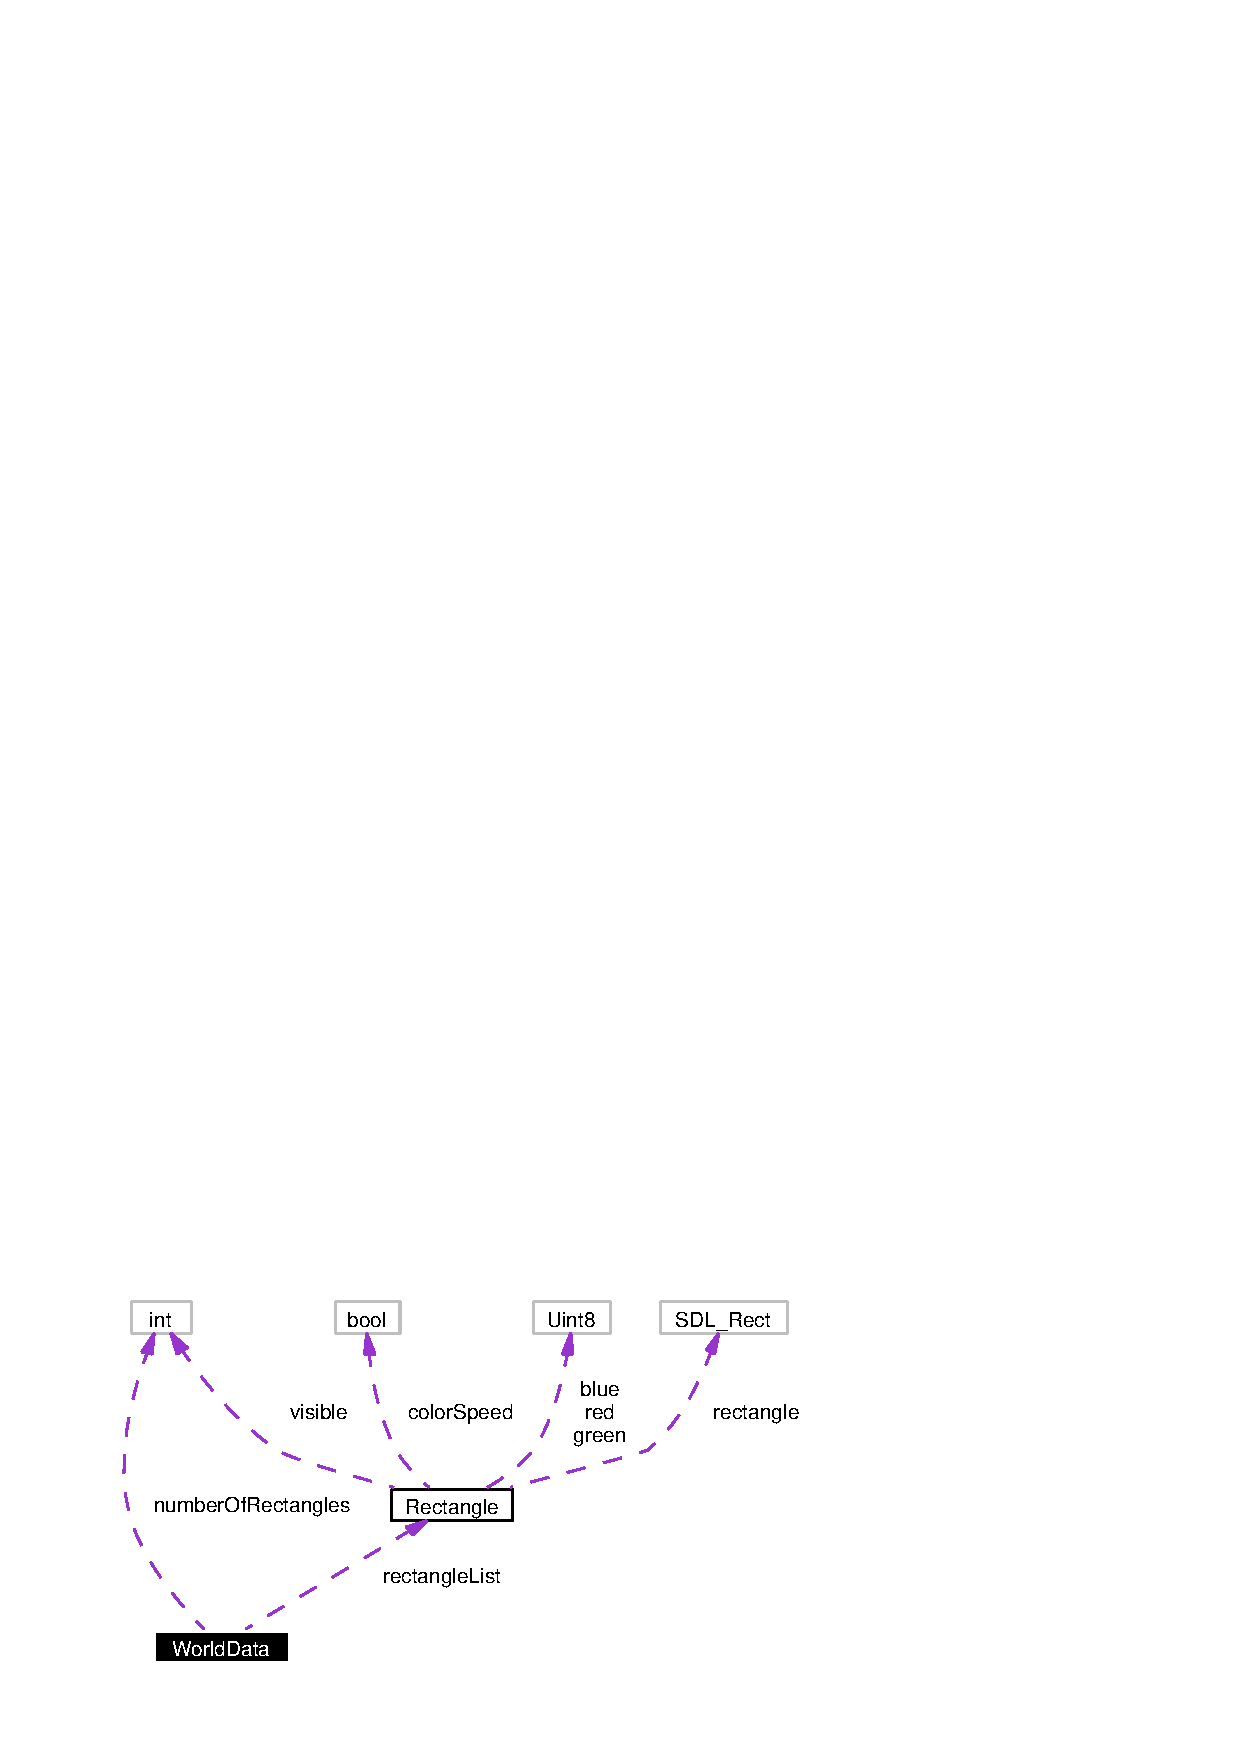
\includegraphics[width=201pt]{classWorldData__coll__graph}
\end{center}
\end{figure}
\subsection*{Public Attributes}
\begin{CompactItemize}
\item 
int {\bf number\-Of\-Rectangles}
\item 
{\bf Rectangle} $\ast$ {\bf rectangle\-List}
\end{CompactItemize}


\subsection{Member Data Documentation}
\index{WorldData@{World\-Data}!numberOfRectangles@{numberOfRectangles}}
\index{numberOfRectangles@{numberOfRectangles}!WorldData@{World\-Data}}
\subsubsection{\setlength{\rightskip}{0pt plus 5cm}int {\bf World\-Data::number\-Of\-Rectangles}}\label{classWorldData_o0}


\index{WorldData@{World\-Data}!rectangleList@{rectangleList}}
\index{rectangleList@{rectangleList}!WorldData@{World\-Data}}
\subsubsection{\setlength{\rightskip}{0pt plus 5cm}{\bf Rectangle}$\ast$ {\bf World\-Data::rectangle\-List}}\label{classWorldData_o1}




The documentation for this class was generated from the following file:\begin{CompactItemize}
\item 
src/{\bf world.hpp}\end{CompactItemize}
